%% appendix

\section{The Equipartition theorem and the Fluctuation dissapation theorem}

\section{Calibration}
The frequency response measurement shown in (?) records the following transfer function in dB of the following:

\begin{equation}
\alpha(f) = \frac{\mathrm{CH2}(f)}{Source}
\end{equation}

Channel

We also know that the error signal spectra of the loop is probed by $CH2(f)$:


\begin{equation}
\mathrm{CH2}(f) = \frac{\mathrm{S}(f)*signal_V}{(1-\mathrm{OLG}(f))}
\end{equation}

Where $signal_V$ is the uncalibrated voltage output from the mixer, $\mathrm{S}(f)$ is the FSS transfer function, and $\mathrm{OLG}(f)$ is the open loop gain of the PDH system.

And we know $\mathrm{OLG}(f) = \mathrm{S}(f)*\mathrm{A}(f)$ so :

\begin{equation}
\mathrm{signal}_m = \mathrm{CH2}(f)*\mathrm{A}(f) \frac{1-\mathrm{OLG}(f)}{\mathrm{OLG}(f)} \frac{L_\mathrm{cav}}{f_\mathrm{laser}}
\end{equation}

Where $\mathrm{A}*(f)$ is the high voltage amplifier response with the Mephisto 2220 laser PZT response. $L_\mathrm{cav}$ is the sample cavity length, $f_\mathrm{laser}$ is the laser frequency. ($\mathrm{signal}_m$)  is the effective cavity length change from the Pockels effect.

Substitute (1) into (4):

\begin{equation}
\mathrm{signal}_m = \mathrm{Source} * \alpha(f) * \mathrm{A}(f) \frac{1-\mathrm{OLG}(f)}{\mathrm{OLG}(f)} \frac{L_\mathrm{cav}}{f_\mathrm{laser}}
\end{equation}

Measured :
Source, $\alpha (f)$, OLG$(f)$, A$(f)$ and $L_\mathrm{cav}$

\section{Laplace calculator / code}

\section{MACOR assembly}

\begin{figure}[H]
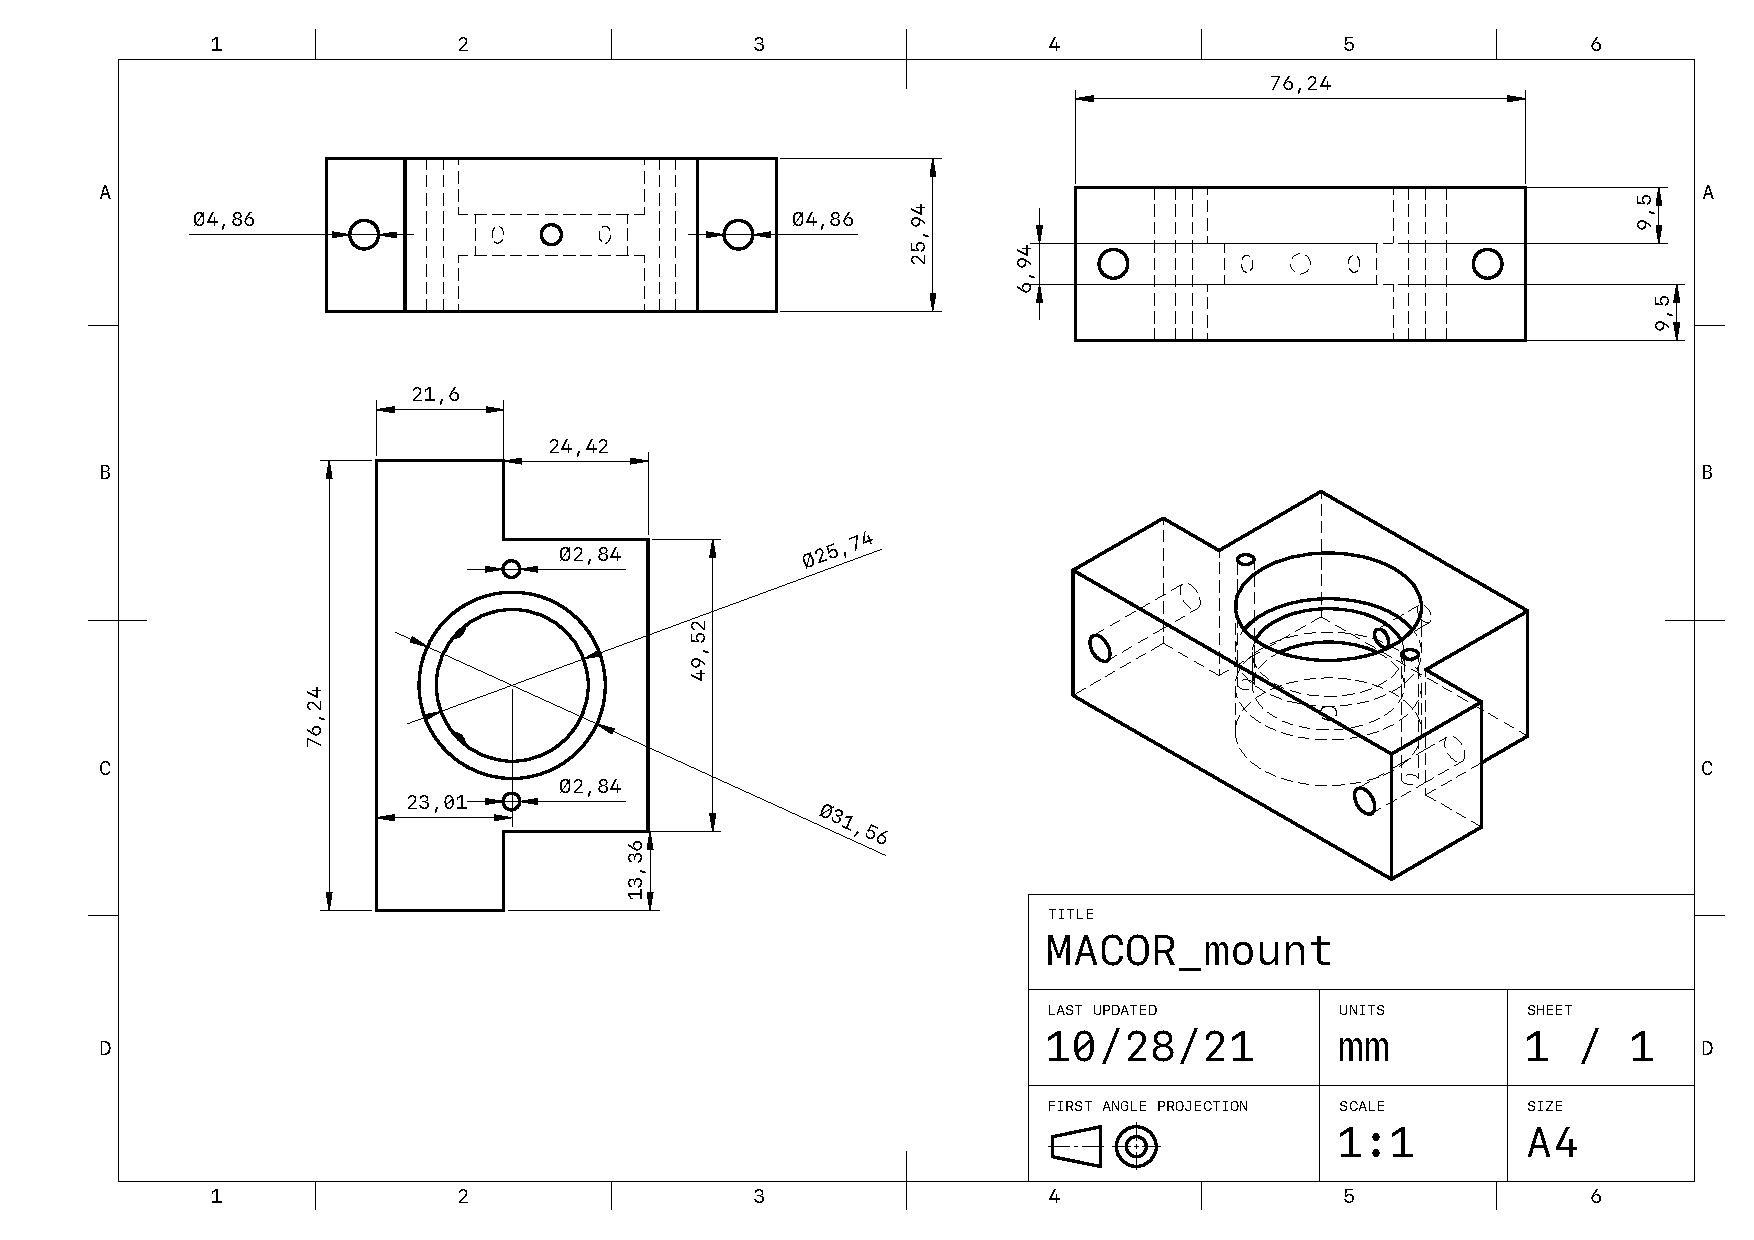
\includegraphics[width=\textwidth]{figs/ALGAAS/MACOR_mount.pdf}
\caption{MACOR mount design constucted in Shapr3D}

\satoshi{First angle projection is used in Europe. In America, third angle projection is used, and I recommend to use it.}

\label{fig:macor_mount_design}
\end{figure}

\section{FSS LTSpice model}

\begin{figure}[H]
\includegraphics[width=\textwidth]{figs/ALGAAS/spice_FSS_tf.png}
\caption{The FSS transfer function simulated in LTspice}
\label{fig:spiceFSS}
\end{figure}
